%   Version 3.0 | Lehrstuhl Produktionsinformatik  |  27.08.2020
%%%%%%%%%  Zusätzlich benötigte Pakete in den Header einfügen  %%%%%%%%%%
%   header.tex
%   Version 1.0     |   Peter Krönes    |   08.05.2018
%%%%%%%%%%%%%%%%%%%%%%%%%%%%%%%%%%%%%%%%%%%%%%%%%%%%%%%%%%%%%%%%%%%%%%%%
\documentclass
[   twoside,         % oneside/twoside : Einseitiger oder zweiseitiger Druck?
    12pt,            % Bezug: 12-Punkt Schriftgröße
    DIV=15,          % Randaufteilung, siehe Dokumentation "KOMA"-Script
    BCOR=17mm,       % Bindekorrektur: Innen 17mm Platz lassen. Copyshop-getestet.
    headsepline,     % Unter Kopfzeile Trennlinie (aus: headnosepline)
    openright,       % Neue Kapitel im zweiseitigen Druck rechts beginnen lassen
    a4paper,         % Seitenformat A4
    listof=totoc,      % Div. Verzeichnisse ins Inhaltsverzeichnis aufnehmen
    bibliography=totoc,        % Literaturverzeichnis ins Inhaltsverzeichnis aufnehmen
]   {scrbook}        %scrbook für Abschlussarbeiten
%%%%%%%%%%%%%%%%%%%%%%%%%%%%%%%%%%%%%%%%%%%%%%%%%%%%%%%%%%%%%%%%%%%%%%%%%
\usepackage[		 % Bibliography
    backend=bibtex,
    natbib=true,
    url=false,
    doi=true,
    eprint=false,
    backref=true
]{biblatex}
\usepackage{hyperref}%[pdftex,bookmarks,colorlinks,citecolor=black,breakl inks]
\appto\UrlBreaks{\do\a\do\b\do\c\do\d\do\e\do\f\do\g\do\h\do\i\do\j
	\do\k\do\l\do\m\do\n\do\o\do\p\do\q\do\r\do\s\do\t\do\u\do\v\do\w
	\do\x\do\y\do\z}						% Umbruch von langen URLs

\DefineBibliographyStrings{ngerman}{%
  backrefpage = {S.},                       % originally "cited on page"
  backrefpages = {S.},                      % originally "cited on pages"
  andothers = {{et\,al\adddot}},
}

%%%%%%%%%%%%%%%%%%%%%         PAKETE        %%%%%%%%%%%%%%%%%%%%%%%%%%%%
\usepackage{fancyhdr}						% Kopf und Fußzeilen
\usepackage[utf8]{inputenc}
\usepackage{csquotes}                       % Anführungszeichen
\usepackage{setspace}                       % Zeilenabstand
\usepackage[ngerman]{babel}                 % Spracheinstellung
\usepackage{float}                          % Platzierung von Objekten
\floatstyle{plaintop}						% Caption über Tabellen
\restylefloat{table}						% ^^^^^^^^^^^^^^^^^^^^
\usepackage{pdfpages}                       % PDF Seitenweise einfügen
\usepackage[font=normalsize]{caption}       % Größe der Bild-/Tabellenunterschrift
\usepackage{acronym}         				% Abkürzungsverzeichnis
\newcommand{\acrosecondcolumn}[1]{
  \acroextra{\makebox[70mm][l]{#1}}
}
\usepackage{graphicx}                       % Für Bilder
\usepackage{subcaption}                     % mehrere Bilder nebeneinander
\usepackage{floatflt}                       % Umlossene Bilder
%\usepackage{overpic}						% Überlagerung von Bildern
\usepackage{svg}                            % Vektorgrafiken im svg-format
%\usepackage{tabu}						    % Abstände in Tabellen (\tabulinesep)
\usepackage{tabularx}                       % Für Tabellen
\usepackage{booktabs}                       % Noch ein Tabellenpaket
\usepackage{color}                          % farbiger Text
\usepackage{lineno}                         % Zeilennummern
\usepackage{microtype}                      % Macht alles schöner
\usepackage{listings}                       % Für Code
\lstset
{ %Formatting for code in appendix
    language=Python,
    basicstyle=\footnotesize,
    numbers=left,
    stepnumber=1,
    showstringspaces=false,
    tabsize=1,
    breaklines=true,
    breakatwhitespace=false,
}
\usepackage{src/mcode/mcode}                % Matlab-Code Paket
\usepackage{src/abkuerzung}                 % Abkürzungen
\usepackage{blindtext}                      % Beispieltext zum auspobieren
\usepackage{todonotes}                      % Fügt Todo Notes ein
\usepackage{eurosym}                        % Eurozeichen mit \euro
\usepackage{afterpage}						% A3 pages in A4 Document
\usepackage{siunitx}
\sisetup{%
     output-decimal-marker = {,},
     inter-unit-product = \ensuremath{{}\cdot{}}
        }
\usepackage{array}                          % Array

%\renewcommand{\familydefault}{\sfdefault}	% set font to arial - funktioniert noch nicht
%\usepackage{arial}


%% Tikz-Pakete
\usepackage{tikz}
\usepackage[siunitx,european,straightvoltages]{circuitikz}          % Schaltkreise
\usetikzlibrary{decorations.pathreplacing}                          % Schaltkreiszusatz
%\usetikzlibrary{arrows.meta}
\usetikzlibrary{arrows}
\usetikzlibrary{patterns}
\usetikzlibrary{ipe}
\usetikzlibrary{positioning}
%\usetikzlibrary{shapes.geometric}
\usetikzlibrary{shapes}
\usetikzlibrary{backgrounds}

%% Mathematik-Pakete für Formeln
\usepackage{amsmath}
\usepackage{amssymb}
\usepackage{amstext}
\usepackage{amsfonts}
\usepackage{mathrsfs}
\usepackage{mathtools}
%\usepackage{esvect}
%\numberwithin{equation}{section} 			% Nummerierungsebene für Gleichungen
\usepackage{gensymb}
\usepackage{multirow}
\usepackage{bigdelim}
\usepackage{epsfig}
\usepackage{etoolbox}
\makeatletter
\patchcmd\Gread@eps{\@inputcheck#1 }{\@inputcheck"#1"\relax}{}{}
\makeatother
%\renewcommand*{\familydefault}{\sfdefault}
%\newcommand*{\head}{\bfseries}
%
\newcolumntype{_}{>{\global\let\currentrowstyle\relax}}
\newcolumntype{^}{>{\currentrowstyle}}
\newcommand{\rowstyle}[1]{\gdef\currentrowstyle{#1}%
	#1\ignorespaces
}

%%%%%%%%%%%%%%%%%%%%%%%%%%%%%%%%%%%%%%%%%%%%%%%%%%%%%%%%%%%%%%%%%%%%%%%%
% Setzt die Kapitel im Anhang nicht ins Inhaltsverzeichnis, setzt man
% Abbildungsverzeichnis und Tabellenverzeichnis hinter den Anhang erscheinen
% diese Trotzdem im Inhaltsverzeichnis.
%\usepackage[toc,page]{appendix}
%%%%%%%%%%%%%%%%%%%%%%%%%%%%%%%%%%%%%%%%%%%%%%%%%%%%%%%%%%%%%%%%%%%%%%%%
\setlength{\parindent}{0pt}                 % Absätze nicht eingerückt
%% Änderungen Pauline %%
\usepackage{cleveref}						% ans Ende verschoben, da Kompilierungsfehler

% Styles um Code mit oder ohne Zeilennummerierung auszugeben
\lstdefinestyle{numbers}{numbers=left, stepnumber=1, numberstyle=\tiny, numbersep=10pt,xleftmargin=1.5em}
\lstdefinestyle{nonumbers}{numbers=none}
\lstdefinelanguage{Python}
{
  morekeywords={from, import, def, return},
  comment=[l]{\#},
  morestring=[b]",
  alsodigit={-},
  alsoletter={&},
}


%% Glossaries für Symbolverzeichnis
\usepackage[acronym,automake]{glossaries}
\usepackage{glossary-longbooktabs}

\newglossary[klg]{konstante}{koi}{kog}{Konstanten}
\newglossary[slg]{symbol}{syi}{syg}{Symbole}

\glsaddkey{unit}{\glsentrytext{\glslabel}}{\glsentryunit}{\GLsentryunit}{\glsunit}{\Glsunit}{\GLSunit}

\newglossarystyle{3colger}{%
    \setglossarystyle{longragged3col}% 				% base this style on the list style
    \renewenvironment{theglossary}{% 				% Change the table type --> 3 columns
     % compute the description width
        \settowidth{\dimen0}{Zeichen}%  			% so viel Platz, wie "Zeichen" braucht
        \settowidth{\dimen2}{laaaaangeEinheit}%
        \setlength{\glsdescwidth}{\linewidth-\dimen0-\dimen2-6\tabcolsep}
        \begin{longtable}{p{\dimen0} p{\glsdescwidth} p{\dimen2}}}%
        {\end{longtable}}%


	% \renewcommand*{\glossaryheader}{%  Change the table header
	%  \bfseries Zeichen & \bfseries Beschreibung & \bfseries Einheit \\
	%           \hline
	%   \vspace{0.05cm}
	%   \endhead}
	\renewcommand*{\glossentry}[2]{%  Change the displayed items
    	\glstarget{##1}{\glossentryname{##1}} %
    	&  \glossentrydesc{##1}
    	& \glsunit{##1}  \tabularnewline
		}
	\renewcommand*{\glsclearpage}{}  % damit alles auf einer Seite bleibt
}


\makeglossaries                                   % activate glossaries-package

\newcommand{\symbolverzeichnis}{
\glsaddall
\setglossarysection{section}
\printglossary[type = symbol, style=3colger]
\printglossary[type = konstante, style=3colger]}


%%%%%%%%%%%%%    Einbinden der Quellen    %%%%%%%%%%%%%%%%%%%%%%%%%%%%%%%
\addbibresource{src/references.bib}

%%%%%%%%%%%%%%%   Folgenden Abschnitt anpassen!    %%%%%%%%%%%%%%%%%%%%%%
% Arbeit
\newcommand{\artderausarbeitung}{Seminararbeit}
\newcommand{\titelderarbeit}{Verbesserung der Pfadplanung am UR5}
% Autor
\newcommand{\namedesautors}{Nik Julin Nowoczyn}
\newcommand{\matrikelnummer}{8529776}
\newcommand{\studiengang}{Ingenieurinformatik}
\newcommand{\pruefer}{Prof.~Dr.-Ing.~Johannes Schilp}
\newcommand{\betreuer}{Ludwig Vogt}
\newcommand{\ausgabedatum}{01.\,10.\,2022}
\newcommand{\abgabedatum}{20.\,02.\,2023}
%%%%%%%%%%%%%%%%%%%%%%%%%%%%%%%%%%%%%%%%%%%%%%%%%%%%%%%%%%%%%%%%%%%%%%%%%
% Hier können eigene Befehle angelegt werden:
%\newcommand{\Name}{Definition}

%%%%%%%%%%%%%%%%%%%%%%%%%%%%%%%%%%%%%%%%%%%%%%%%%%%%%%%%%%%%%%%%%%%%%%%%%
\begin{document}
    \onehalfspacing
    % Wird auf alle nicht leeren Seiten angewandt
% siehe auch;
% http://tug.ctan.org/tex-archive/macros/latex/contrib/fancyhdr/fancyhdr.pdf
\fancypagestyle{title}{%
	\fancyhf{}
	\fancyhead[L]{Fakultät für Angewandte Informatik \\
		\textbf{Lehrstuhl für Produktionsinformatik} \\ Prof. Dr.-Ing. Johannes Schilp}

	\fancyhead[R]{
		\raisebox{0pt}[0pt][0pt]{
\includegraphics[width=3.5cm]{src/Uni_Aug_Logo_Basis_pos_A.pdf}}
	}

	\renewcommand{\headrulewidth}{0.4pt} %obere Trennlinie
}


\renewcommand{\chaptermark}[1]{\markboth{
		\thechapter. #1}{}}
%\renewcommand{\sectionmark}[1]{\markboth{
%		\thesection. #1}{}}


\pagestyle{fancyplain}% <- pagestyle fancyplain
\renewcommand\plainheadrulewidth{.4pt}% headrule on plain pages
\fancyhf{}
\fancyhead[L]{\namedesautors}
\fancyhead[R]{\leftmark}
%\fancyhead[R]{\rightmark}
\fancyfoot[RE,LO]{}
\fancyfoot[LE,RO]{\pagemark}
\renewcommand{\chaptermark}[1]{%
	\markboth{#1}{}}


\headsep = 20pt % COOLER CODE: Das Ding setzt die Margin zwischen Header und Text darunter
				% Bei Überschriften setzt sich diese Margin aber aus dieser bottom Margin + der
				% top Margin von Überschriften zusammen. Diese kann mit dem folgenden Command
				% geändert werden:
\renewcommand*{\chapterheadstartvskip}{\vspace*{0cm}} % COOLER CODE:
													  % Setzt top Margin bei \chapter. Wenn dus
													  % so haben willst wie vorher, einfach die
													  % Zeile löschen. Selbe gilt bei \headsep

%%  Der Vollständigkeithalber die alten verschiedenen Pagestyles von Peter
%   pagestyle.tex
%   Version 1.0     |   Peter Krönes    |   08.05.2018

%%%%%%%%%%%%%%%%%%%%%%%  PAGESTYLE  %%%%%%%%%%%%%%%%%%%%%%%%%%%%%%%%%%%%
%
%\usepackage{fancyhdr}
%\pagestyle{fancy}
%\renewcommand{\chaptermark}[1]{\markboth{
%		\thechapter. #1}{}}
%\renewcommand{\sectionmark}[1]{\markboth{
%		\thesection. #1}{}}
%
%%%%%%%%%%%%%%%%%%%%%%%%%%%%%%%%%%%%%%%%%%%%%%%%%%%%%%%%%%%%%%%%%%%%%%%%
%\fancypagestyle{scrheadings}{
%	\fancyhead[LE,RO]{\nouppercase\leftmark} 	% Kapitelname oben ins andere Eck
%	\fancyhead[LO,RE]{\namedesautors}	% Autor oben im Eck
%	\fancyfoot[LE,RO]{\pagemark} 		% Seitenzahl unten im Eck
%	\fancyfoot[C]{}
%}
%%%%%%%%%%%%%%%%%%%%%%%%%%%%%%%%%%%%%%%%%%%%%%%%%%%%%%%%%%%%%%%%%%%%%%%%
% Pagestyle für die erste Seite der List of Figures/Tables
%\fancypagestyle{pagenumberstyle}{
%	\renewcommand{\headrulewidth}{0pt}
%
%	\fancyhead[LE,RO]{\chaptermark} 	% Kapitelname oben ins andere Eck
%	\fancyhead[LO,RE]{\namedesautors}	% Autor oben im Eck
%	\fancyfoot[LE,RO]{\pagemark} 		% Seitenzahl unten im Eck
%	\fancyfoot[C]{}
%}
% Unterscheidung zwischen einseitig und zweiseitigem Druck nicht nötig, da Kapitel bei zweiseitigem Druck immer rechts anfangen.
%%%%%%%%%%%%%%%%%%%%%%%%%%%%%%%%%%%%%%%%%%%%%%%%%%%%%%%%%%%%%%%%%%%%%%%%
%
%%%%%%%%%%%%%%%%%%%%%%%%%%%%%%%%%%%%%%%%%%%%%%%%%%%%%%%%%%%%%%%%%%%%%%%%
% Pagestyle für scrartcl
%\fancypagestyle{articlestyle}{
%	\renewcommand{\headrulewidth}{0.1pt}
%	\fancyhead[LE,RO]{\chaptermark} 	% Kapitelname oben ins andere Eck
%	\fancyhead[LO,RE]{\namedesautors}	% Autor oben im Eck
%	\fancyfoot[LE,RO]{\pagemark} 		% Seitenzahl unten im Eck
%	\fancyfoot[C]{}
%}
% Unterscheidung zwischen einseitig und zweiseitigem Druck nicht nötig, da Kapitel bei zweiseitigem Druck immer rechts anfangen.
%%%%%%%%%%%%%%%%%%%%%%%%%%%%%%%%%%%%%%%%%%%%%%%%%%%%%%%%%%%%%%%%%%%%%%%%



%% wurde dann vor listoffigures, listoftables, tableofcontents und printbibliography
%% wie folgt eingestellt: \tableofcontents{\thispagestyle{pagenumberstyle}}

    %   titlepage.tex

\begin{titlepage}
\thispagestyle{title}


\vspace*{65mm}

\centering
{\Huge \textbf{\artderausarbeitung}}\\[5ex]
{\Large \textbf{\titelderarbeit}}\\[5ex]

\vspace{35mm}

\flushleft
\begin{tabular}{ll}
Vorgelegt von:          & \quad \namedesautors \\[1,5ex]
Matrikelnummer:			& \quad \matrikelnummer \\[1,5 ex]
Studiengang:            & \quad \studiengang \\[1,5ex]
Prüfer:					& \quad \pruefer \\[1,5ex]
Betreuer:				& \quad \betreuer \\[1,5ex]
Ausgabedatum:           & \quad \ausgabedatum \\[1,5ex]
Abgabedatum:            & \quad \abgabedatum\\[1,5ex]
\end{tabular}
\vfill
\end{titlepage}
\cleardoublepage

    \pagenumbering{Roman}
    \onehalfspacing
    \chapter*{Aufgabenstellung}
\addcontentsline{toc}{chapter}{Aufgabenstellung}
\chaptermark{Aufgabenstellung}

    \chapter*{Kurzfassung}
\addcontentsline{toc}{chapter}{Kurzfassung}
\chaptermark{Kurzfassung}


In dieser Arbeit wird die Steuerung des UR5 näher untersucht und eine Ursache der häufig auftretenden Selbstkollisionen ermittelt.
Zudem werden alternative Algorithmen erläutert und die Vor- und Nachteile der verschiedenen Methoden verglichen.
Dabei wird eine direkte und schnelle Berechnungsmethode zur Bestimmung der Gelenkwinkel vorgestellt und die auftretenden Selbstkollisionen durch dadurch begründet, dass die Software des UR5 vermutlich stattdessen auf einer numerischen Methode der inversen Kinematik basiert.
Es wird festgestellt, dass für jede Endeffektor-Transformation in der Regel bis zu acht mögliche Roboterstellungen existieren und ein Algorithmus vorgestellt,
der ohne komplizierte Pfadplanung alle Lösungswege für eine gerade Bahn berechnen und auf Kollision überprüfen kann.
    \tableofcontents        % Inhaltsverzeichnis
    \listoffigures        % Abb.verzeichnis
    \listoftables        % Tabellenverzeichnis
    \chapter*{Abkürzungsverzeichnis}

\begin{acronym}
 \setlength{\itemsep}{-0.5cm}
 \acro{dhkonv}[DH-Konvention]{Denavit-Hartenberg-Konvention}
 \acro{urdf}[URDF]{Unified Robot Description Format}
 \acro{ros}[ROS]{das Robot Operating System}
 \acro{rrt}[RRT]{Rapidly Exploring Random Tree}
\end{acronym}

% see usage here: https://ramibaddour.com/2017/01/18/latex-working-with-acronyms/
%%%%%%%%%%%%%%%%%%%%%%%%%%%%%%%%%%%%%%%%%%%%%%%%%%%%%%
% zum Ausgeben der Verzeichnisse
%\symbolverzeichnis

    \cleardoublepage
    \pagenumbering{arabic}
%%%%%%%%%%%%%%     Eigene Kapitel hier einfügen    %%%%%%%%%%%%%%%%%%%%%%
%    \input{010_Räumliche_Beschreibungsformalismen}
    \cleardoublepage


\chapter{Direkte Kinematik}\label{ch:direkte-kinematik}

Die direkte Kinematik ist dafür verantwortlich, aus den verschiedenen Winkeln und Positionen der Gelenke die Rotation und Position des Endeffektors im Raum zu berechnen.
Dazu wird zunächst in jedem Gelenk ein Koordinatenursprung gelegt, der eine Nullstellung jedes Gelenks beschreibt.
Um alle Gelenke in einer kinematischen Kette abzubilden, kann mit einem Parameter in den Freiheitsgraden des entsprechenden Gelenks eine Rechenvorschrift aufgebaut werden, um den Roboter zu beschreiben und die Position des Endeffektors schnell bestimmen zu können.

Zur Beschreibung von Transformationen wird in dieser Arbeit auf die Homogene Transformationsmatrix zurückgegriffen.
Diese besteht aus einer Rotationsmatrix $R_{a,b}$, die die Rotation von System $a$ in System $b$ beschreibt und einem Translationsvektor $P_{a,b}$, der die Translation zwischen den zwei Systemen entspricht~\ref{eq:inv-rule0}~\cite[28]{craigIntroductionRoboticsMechanics2009}.
Um eine Inverse Transformation von System $b$ in System $a$ zu erhalten, kann die Inverse der Transformationsmatrix $T_{a,b}$ oder die Regel aus Gleichung~\ref{eq:inv-rule1} verwendet werden.
Bei der Multiplikation zweier geeigneter Matrizen können mehrere Transformationen in einer Matrix dargestellt werden.
Ein Beispiel hierfür findet sich in Gleichung~\ref{eq:inv-rule2}.

?? verschieben in Abschnitt 1.4 ??

\begin{equation}
    T_{a,b} = \begin{bmatrix}
                  R_{a,b} & P_{a,b} \\
                  0^T     & 1
    \end{bmatrix} \label{eq:inv-rule0}
\end{equation}
\begin{equation}
    T_{b,a} = \left( T_{a,b} \right)^{-1} =
    \begin{bmatrix}
        \left(R_{a,b}\right)^T & - \left(R_{a,b}\right)^T P_{a,b} \\
        0^T     & 1
    \end{bmatrix} =
    \begin{bmatrix}
        R_{b,a} & - R_{b,a}P_{a,b} \\
        0^T     & 1
    \end{bmatrix}
    \label{eq:inv-rule1}
\end{equation}
\begin{equation}
    T_{a,b}\cdot T_{b,c}=T_{a,c}    \label{eq:inv-rule2}
\end{equation}


\section{DH-Konvention}\label{sec:dh-konvention}

?? Quelle


Um Rotation und Translation eines Gliedes der kinematischen Kette darzustellen kann die sog.\ DH-Konvention oder auch DH-Transformation verwendet werden.
Diese Konvention beschreibt ein standardisiertes Vorgehen wie die Transformation des nächsten Gelenks im Koordinatensystem des momentanen Gelenks ausgedrückt werden soll~\cite{denavitKinematicNotationLowerPair1955,craigIntroductionRoboticsMechanics2009}.
Es gelten die folgenden Regeln:

\begin{enumerate}
    \item Achse $z_{n}$ liegt entlang der Bewegungsachse des Gelenks $n$
    \item Achse $x_{n}$ liegt auf der kürzesten Verbindung zwischen Achsen $z_{n-1}$ und $z_{n}$.
    \item Die $y_{n}$ Achse wird rechtshändig ergänzt.
\end{enumerate}

Dabei sind die Ursprünge der Gelenkkordinatensysteme oftmals nicht im Gelenkursprung, was Komplexität für die Berechnung von Transformationen verringert.
Aus der Beziehung der zwei Koordinatensysteme können die DH-Parameter abgeleitet werden (siehe auch Abbildung~\ref{fig:dh-konvention1}):

\begin{itemize}
    \item $\theta_n$ Winkel zwischen $x_{n-1}$ und $x_n$ mit Rotationsachse $z_{n-1}$
    \item $d_n$: Kleinster Abstand zwischen $x_{n-1}$ und $x_n$
    \item $a_n$: Abstand zwischen den Achsen $z_{n-1}$ und $z_n$
    \item $\alpha_n$ Winkel zwischen $z_{n-1}$ und $z_n$ mit Rotationsachse $x_{n}$
\end{itemize}

Dies entspricht den folgenden Transformationsmatrizen (Gleichungen~\ref{eq:dh1},~\ref{eq:dh2},~\ref{eq:dh3},~\ref{eq:dh4}):

\newcommand{\ct}{\cos(\theta_n)}
\newcommand{\st}{\sin(\theta_n)}
\newcommand{\ca}{\cos(\alpha_n)}
\newcommand{\sa}{\sin(\alpha_n)}

\begin{equation}
    T_{\theta_n} =
    \begin{bmatrix}
        \ct & -\st & 0 & 0 \\
        \st & \ct  & 0 & 0 \\
        0   & 0    & 1 & 0 \\
        0   & 0    & 0 & 1 \\
    \end{bmatrix}
    \label{eq:dh1}
\end{equation}
\begin{equation}
    T_{d_n} =
    \begin{bmatrix}
        1 & 0 & 0 & 0   \\
        0 & 1 & 0 & 0   \\
        0 & 0 & 1 & d_n \\
        0 & 0 & 0 & 1   \\
    \end{bmatrix}
    \label{eq:dh2}
\end{equation}

\begin{equation}
    T_{a_n} =
    \begin{bmatrix}
        1 & 0 & 0 & a_n \\
        0 & 1 & 0 & 0   \\
        0 & 0 & 1 & 0   \\
        0 & 0 & 0 & 1   \\
    \end{bmatrix}
    \label{eq:dh3}
\end{equation}

\begin{equation}
    T_{\alpha_n} =
    \begin{bmatrix}
        1 & 0   & 0    & 0 \\
        0 & \ca & -\sa & 0 \\
        0 & \sa & \ca  & 0 \\
        0 & 0   & 0    & 1 \\
    \end{bmatrix}
    \label{eq:dh4}
\end{equation}

Um nun Koordinatensystem $n-1$ in Koordinatensystem $n$ zu überführen, kann die Transformationsmatrix $T_{n-1,n}$ verwendet werden (Gleichung~\ref{eq:dh5}).
Für den beweglichen Freiheitsgrad der Gelenke wird dann jeweils eine freie Variable festgelegt ($\theta_n$ für translatorische und $d_n$ für rotatorische Gelenke).

\begin{equation}
    T_{n-1,n}(\theta_n, d_n) \coloneqq T_{\theta_n} \cdot T_{d_n} \cdot T_{a_n} \cdot T_{\alpha_n} =
    \begin{bmatrix}
        \ct & -\st\ca & \st\sa  & a_n\ct \\
        \st & \ct\ca  & -\ct\sa & a_n\st \\
        0   & \sa     & \ca     & d_n    \\
        0   & 0       & 0       & 1      \\
    \end{bmatrix}
    \label{eq:dh5}
\end{equation}

\begin{figure}[h]
    \centering
    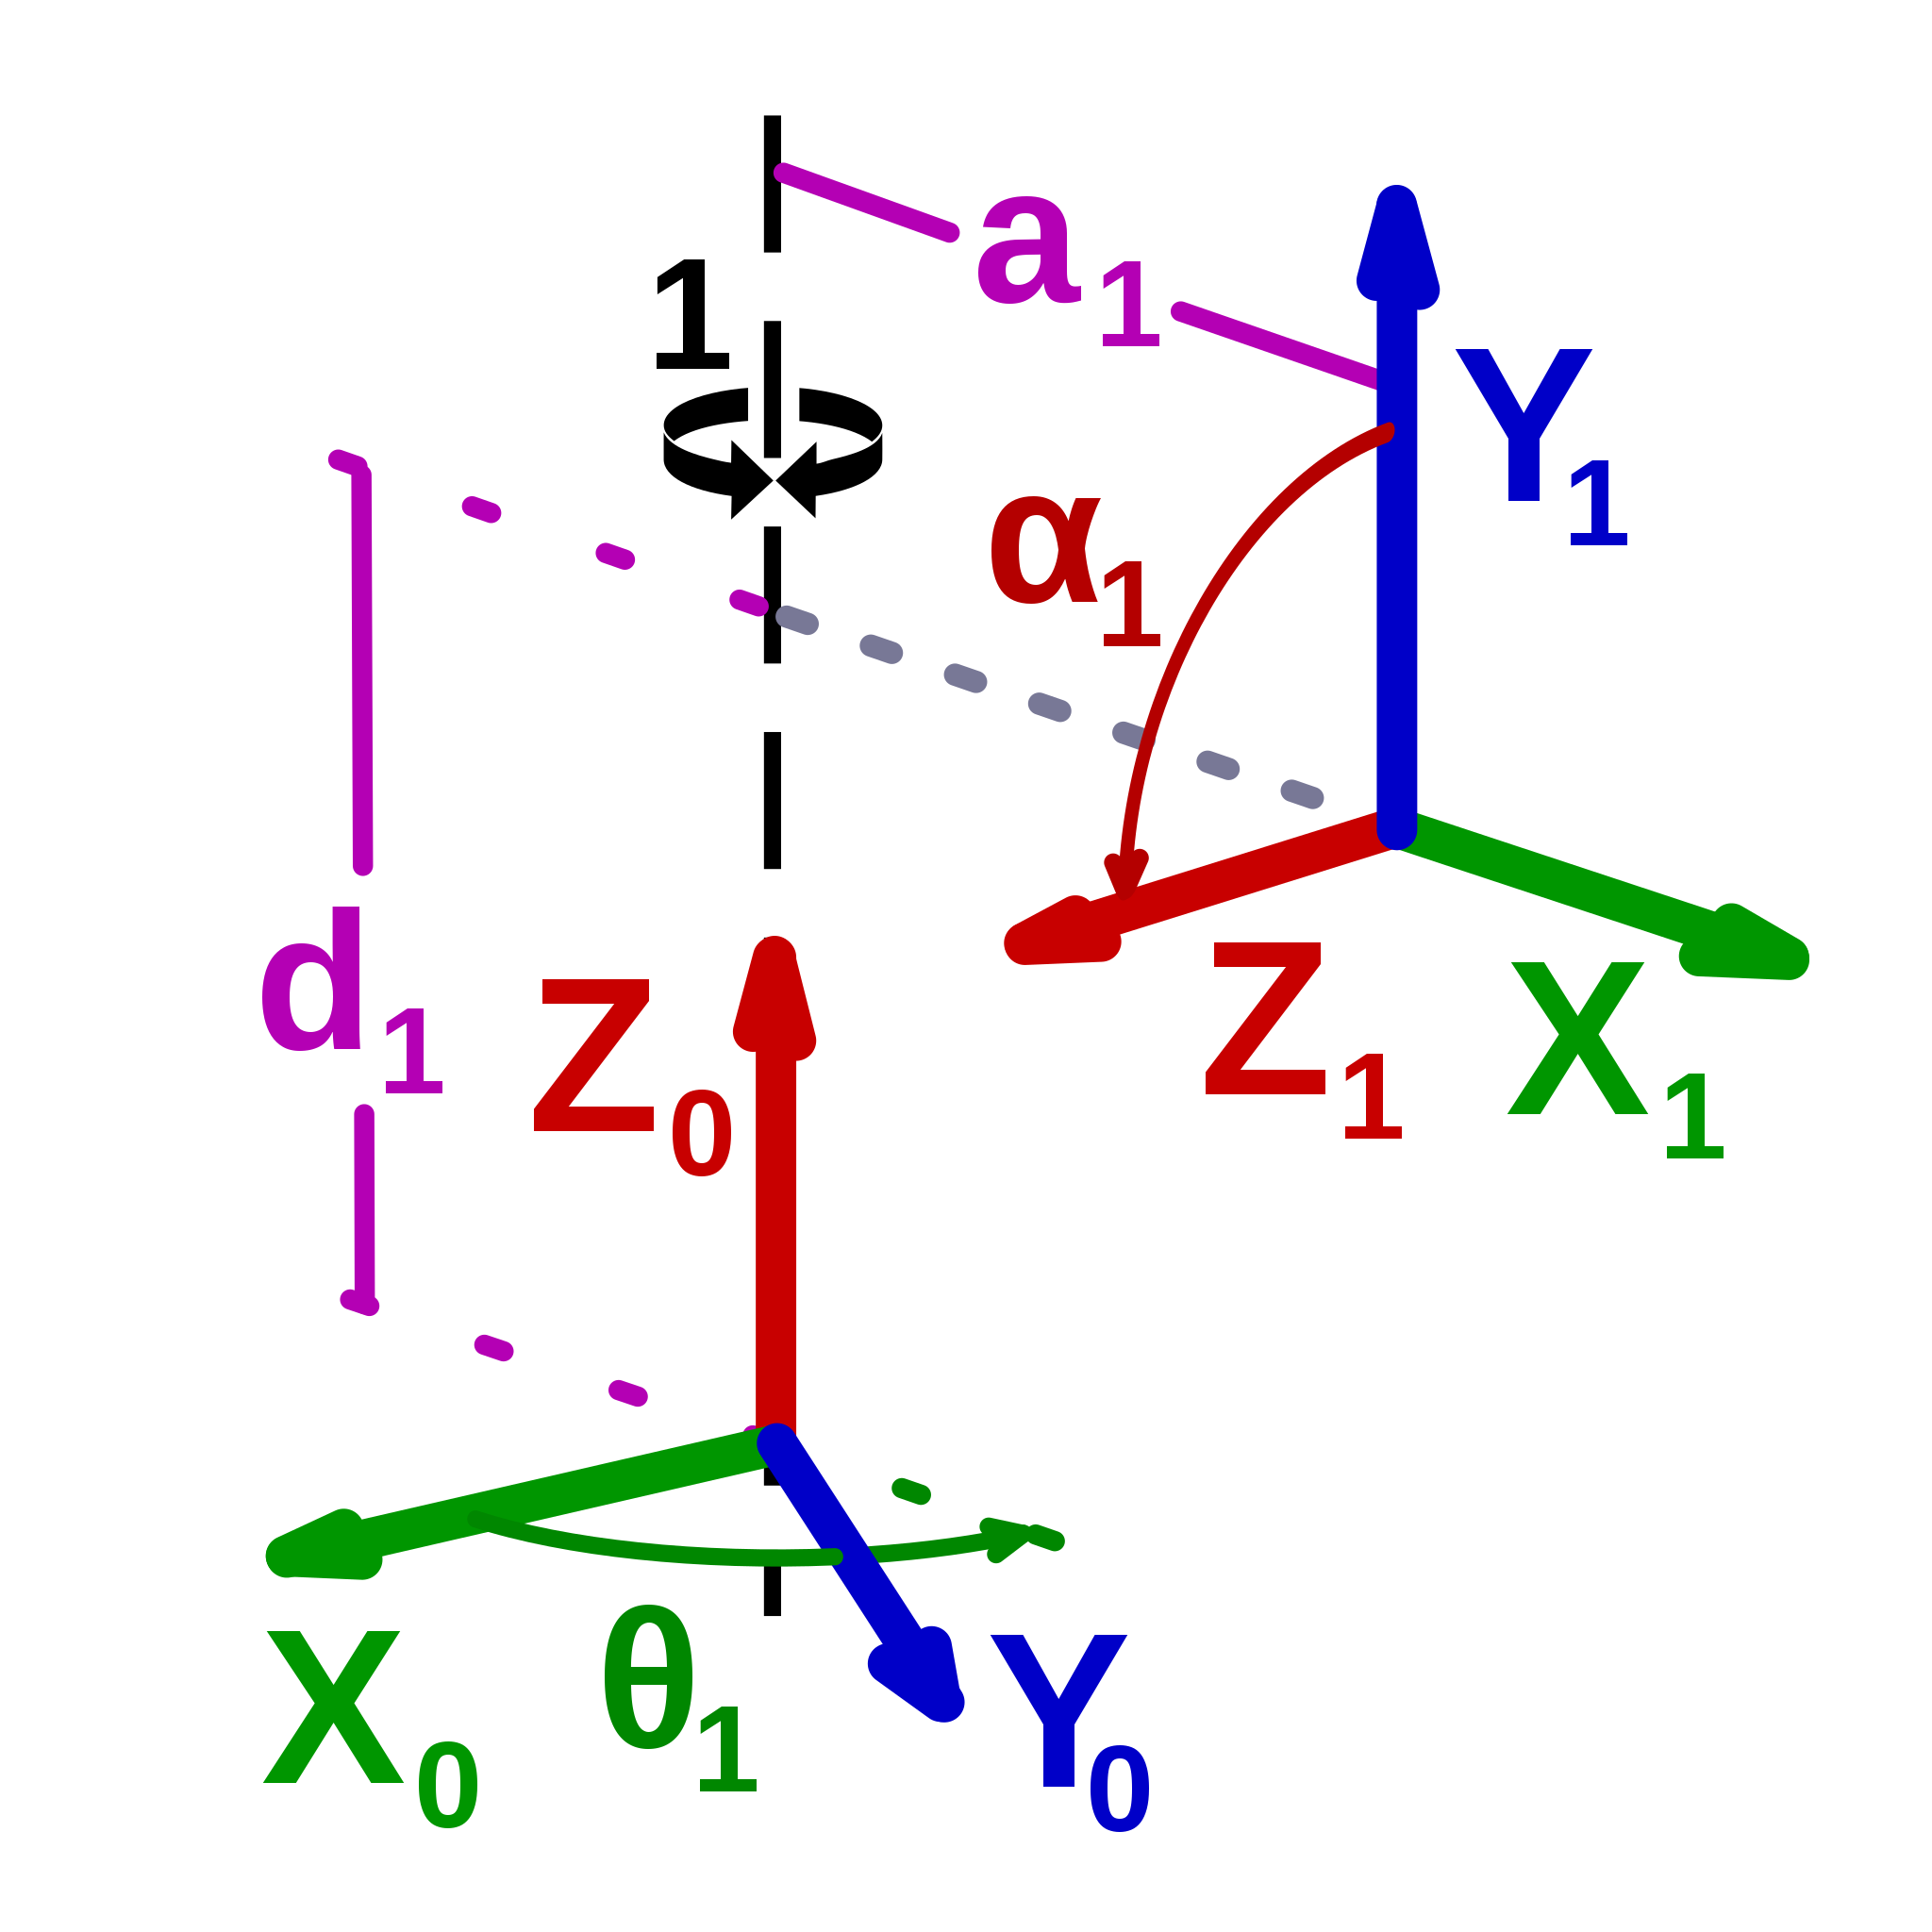
\includegraphics[width = .5\textwidth]{Bilder/Denavit-Hartenberg-Transformation.svg}
    \caption{DH-Konvention zwischen zwei Gelenken~\cite{jahobrCoordinateSystemsDenavitHartenberg2007}}\label{fig:dh-konvention1}
\end{figure}

Oftmals wird in der Literatur auch eine alternative, modifizierte Form der DH-Parameter verwendet~\cite[75]{craigIntroductionRoboticsMechanics2009}.
Um die Vergleichbarkeit mit~\cite{rasmusandersenKinematicsUR52018} zu gewährleisten wird in der Rechnung sowie im Code diese alternative Methode eingesetzt.
Dabei verändert sich die Transformationsmatrix eines Gelenks auf die Werte aus Gleichung~\ref{eq:alt-tf}:

\begin{equation}
    T_{n-1,n}(\theta_n, d_n) \coloneqq
    \begin{bmatrix}
        \ct                   & -\st                  & 0                   & a_{n-1}                  \\
        \st\cos(\alpha_{n-1}) & \ct\cos(\alpha_{n-1}) & -\sin(\alpha_{n-1}) & -d_{n}\sin(\alpha_{n-1}) \\
        \st\sin(\alpha_{n-1}) & \ct\sin(\alpha_{n-1}) & \cos(\alpha_{n-1})  & d_{n}\cos(\alpha_{n-1})  \\
        0                     & 0                     & 0                   & 1                        \\
    \end{bmatrix}
    \label{eq:alt-tf}
\end{equation}


\section{Unified Robot Description Format}\label{sec:urdf}

Das \ac{urdf} ist ein Standard, entwickelt für \ac{ros}, der sowohl die geometrischen als auch physischen und visuellen Eigenschaften eines Roboters beschreiben kann.
Dafür ist eine auf XML basierende Datei nötig, die mithilfe von XML-Tags den Roboter aus sog. \enquote{Links} und \enquote{Joints} aufbaut~\cite{ros.orgUrdfXMLModel}.

Links sind die physischen Verbindungen zwischen zwei Gelenken und können verschiedene Eigenschaften aufweisen.
Neben den dem geometrischen Aufbau wird zudem unterschieden zwischen visuellen Eigenschaften (\enquote{visual}), Kollisionseigenschaften (\enquote{collision}) und Trägheitseigenschaften (\enquote{inertial}).

Joints sind Gelenke, die aus der Verbindung zweier physischer Links bestehen.
Dabei sind nicht nur translatorische (\enquote{prismatic}) und rotatorische Gelenke (\enquote{revolute}) beschreibbar, sondern auch feste (\enquote{fixed}), schwebende (\enquote{floating}) und planare Verbindungen (\enquote{planar}).
Für die Beschreibung eines Joints wird der vorhergehende Link als \enquote{parent} und der nächste Link als \enquote{child} bezeichnet.
Zudem müssen im Feld \enquote{origin} Translation und Rotation des Ursprungs im Koordinatensystem des Parent Links, sowie im Feld \enquote{axis} je nach Gelenk die Rotationsachse, Translationsachse oder Normale der Bewegungsoberfläche angegeben werden.
Desweiteren ist es möglich, Schnittstellen für die Bewegung der Motoren zu definieren und Bewegungslimits für die Gelenke anzugeben, um die Ansteuerung des Roboters und die Bewegungsplanung zu vereinfachen.

Die Schritte zur Berechnung der direkten Kinematik können für das bessere Verständnis im Code ?? (Anhang referenz) direkt nachvollzogen und visualisiert werden.


\section{Beschreibung des UR5}\label{sec:ur5-in-dh}
Der in dieser Arbeit betrachtete Roboter ist der UR5e von Universal Robots.
Dieser ist ein vergleichsweise günstiger Roboter mit verringerter Zahl an Singularitäten (siehe Abschnitt~\ref{sec:singularitaten}), sechs Gelenken und einer offenen kinematischen Kette.
Offiziell wird der Roboter mit den DH-Parametern aus Tabelle~\ref{tab:ur5-dh1} und dynamischen Eigenschaften der Links aus Tabelle~\ref{tab:ur5-dh2} beschrieben~\cite{universalrobotsUniversalRobotsDH}.
Abbildung~\ref{fig:ur5-axis} kann zudem die Dimensionierung des Roboters und die Anordnung der Achsen in Nullstellung entnommen werden.

Nach Datenblatt~\cite{universalrobotsUR5TechnicalSpecifications} hat der UR5 einen Arbeitsraum mit Radius 85cm (Abstand vom Befestigungspunkt bei ausgestrecktem Arm) und kann sich mit einer Maximalgeschwindigkeit von bis zu 180°/s bewegen.

\begin{figure}[h]
    \centering
    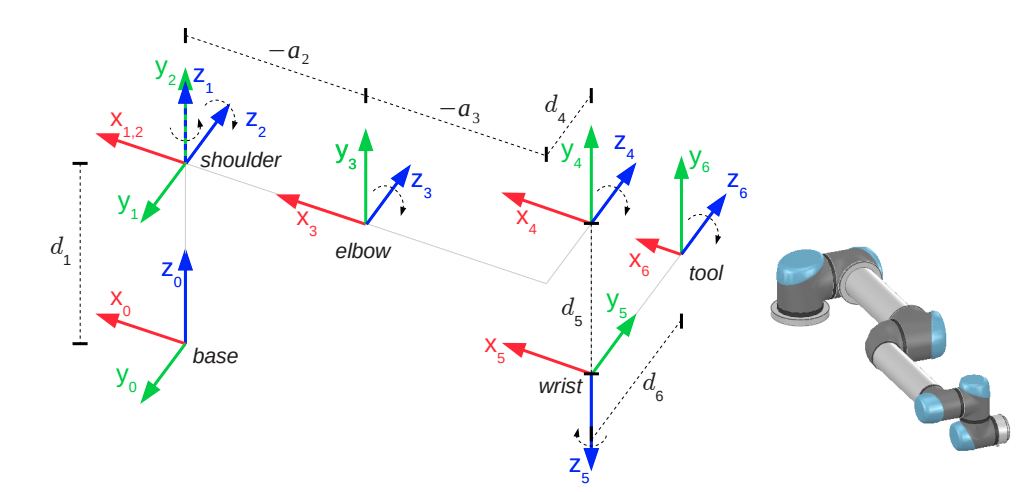
\includegraphics[width = .9\textwidth]{Bilder/ur5-axis}
    \caption{Achsen des UR5-Roboters mit Angabe der DH-Parameter (links) und Visualisierung der Nullposition (rechts)~\cite{rasmusandersenKinematicsUR52018}}\label{fig:ur5-axis}
\end{figure}

\begin{table}
    \centering
    \begin{tabular}{lrrrllrl}
        \toprule
        \textbf{Joint} & $\boldsymbol{\theta}$ \textbf{[rad]} & $\boldsymbol{a}$ \textbf{[m]} & $\boldsymbol{d}$ \textbf{[m]} & $\boldsymbol{\alpha}$ \textbf{[rad]}  \\
        \midrule
        Joint 1        & 0                                    & 0                             & 0.089159                      & \pi/2                                \\
        Joint 2        & 0                                    & -0.425                        & 0                             & 0                                    \\
        Joint 3        & 0                                    & -0.3922                       & 0                             & 0                                    \\
        Joint 4        & 0                                    & 0                             & 0.10915                       & \pi/2                                \\
        Joint 5        & 0                                    & 0                             & 0.09465                       & -\pi/2                               \\
        Joint 6        & 0                                    & 0                             & 0.0823                        & 0                                    \\
        \bottomrule
    \end{tabular}
    \caption{DH-Parameter des UR5e Roboters von Universal Robots~\cite{universalrobotsUniversalRobotsDH}}
    \label{tab:ur5-dh1}
\end{table}
\begin{table}
    \centering
    \begin{tabular}{lrrrllrl}
        \toprule
        \textbf{Link} & \textbf{Masse [kg]} & \textbf{Schwerpunkt [m]} \\
        \midrule
        Link 1        & 3.7                 & [0, -0.02561, 0.00193]   \\
        Link 2        & 8.393               & [0.2125, 0, 0.11336]     \\
        Link 3        & 2.33                & [0.15, 0.0, 0.0265]      \\
        Link 4        & 1.219               & [0, -0.0018, 0.01634]    \\
        Link 5        & 1.219               & [0, 0.0018,0.01634]      \\
        Link 6        & 0.1879              & [0, 0, -0.001159]        \\
        \bottomrule
    \end{tabular}
    \caption{Beschreibung der dynamischen Eigenschaften des UR5e Roboters von Universal Robots~\cite{universalrobotsUniversalRobotsDH}}
    \label{tab:ur5-dh2}
\end{table}


\section{Geschwindigkeitskinematik}

Um einen Roboter in Bewegung darzustellen, ist nicht nur die Transformation der Gelenke relevant, sondern auch dessen Kinematik und Dynamik.
Dies ist besonders relevant, da in der echten Welt bestimmte Maximalwerte für (Winkel-) Geschwindigkeit und Beschleunigung, sowie Trägheit und Drehmoment eingehalten werden müssen, um den sicheren Betrieb sowie das Verhalten der Masse korrekt abzubilden.

Für die Berechnung der Geschwindigkeit des Endeffektors im Gelenk $e$ kann die Jakobi-Matrix verwendet werden.
Dabei gilt für eine Drehung nach DH-Konvention um Achse $z_{n-1}$ für die Geschwindigkeit Gleichung~\ref{eq:kin-1} und für die Winkelgeschwindigkeit Gleichung~\ref{eq:kin-2}.
Für translatorische Gelenke gelten stattdessen Gleichungen~\ref{eq:kin-1-1} und~\ref{eq:kin-2-1}.
Die Vektoren $z_{i}$ entsprechen jeweils der Einheitsvektor der z-Achse $z_{i} = \frac{Z_{0,i}}{\lvert Z_{0,i} \rvert}$ auf Basis der Transformationsmatrix $T_{0,i} = \prod_{n=1}^{i}T_{n-1,n}$ (siehe Konvention Gleichung~\ref{eq:inv-konv}).

\begin{equation}
    J_{P_{n}} = z_{n-1} \times (P_{e} - P_{n-1}) \label{eq:kin-1}
\end{equation}
\begin{equation}
    J_{\omega_{n+1}} = z_{n-1} \label{eq:kin-2}
\end{equation}
\begin{equation}
    J_{P_{n}} = z_{n-1} \label{eq:kin-1-1}
\end{equation}
\begin{equation}
    J_{\omega_{n+1}} = 0 \label{eq:kin-2-1}
\end{equation}

Für alle Gelenke ergibt sich dann für die Jakobi-Matrix eines Sechs-Achsen-Roboters wie dem UR5 die folgende Gleichung~\ref{eq:kin-3} mit jeweils sechs Spalten und Zeilen.
Um die Geschwindigkeit des Endeffektors $v_6$ zu erhalten, muss die Matrix mit der Geschwindigkeit $\dot{\theta}$ multipliziert werden (Gleichung~~\ref{eq:kin-4}).

\begin{equation}
    J_{0,6}=
    \begin{pmatrix}
        J_{P_1}      & \dots & J_{P_6}      \\
        J_{\omega_1} & \dots & J_{\omega_6}
    \end{pmatrix}\label{eq:kin-3}
\end{equation}
\begin{equation}
    v_6 =
    \begin{pmatrix}
        \dot{P}_{0,6} \\ \omega_6
    \end{pmatrix} =
    J_{0,6}\cdot\dot{\theta}
    \label{eq:kin-4}
\end{equation}
    \cleardoublepage


\chapter{Inverse Kinematik}

In der direkte Kinematik wird aus den Gelenkzuständen Position und Rotation des Endeffektors bestimmt.
Der umgekehrte Vorgang, also das Berechnen der Gelenkpositionen bei gegebener Zieltransformation, wird als inverse Kinematik bezeichnet.
Dies ist erforderlich, um Aufgaben in der Umgebung des Roboters zu lösen und die angestrebten Zielpunkte zu erreichen.
Dabei muss beachtet werden, dass oft mehrere gleichwertige Lösungen für eine Zielstellung des Endeffektors vorliegen.
Allerdings kann die inverse Kinematik offener Ketten oft nicht einfach direkt mithilfe einer mathematischen Formel gelöst werden (siehe Abschnitt~\ref{sec:analytische-losung}).
Im Fall des UR5, ist dies allerdings in den meisten Fällen möglich.

Die Lösung des Problems kann geometrisch, analytisch oder numerisch gelöst werden.
Auf die ersten beiden Lösungsmöglichkeiten wird im Folgenden näher eingegangen.


\section{Analytische Lösung}\label{sec:analytische-losung}

Für eine direkte Lösung muss zunächst die Formel aus Gleichung~\ref{eq:dh5} oder~\ref{eq:alt-tf} herangezogen werden.
Nach Multiplikation der Transformationsmatrizen müsste die entstehende Gleichung~\ref{eq:inv-kin1} nach den freien Variablen $\theta_1$ bis $\theta_n$ bzw. $d_1$ bis $d_n$ aufgelöst werden.
Da aufgrund der rotatorischen Gelenke nichtlineare trigonometrische Funktionen verwendet werden, ist diese Funktion bei Industrierobotern überwiegend nichtlinear und in vielen Fällen auch nicht lösbar.

\begin{equation}
    T_{0,n}(\overrightarrow{q}) = \prod_{i=1}^{n} T_{i-1,i}(q_i)     \label{eq:inv-kin1}
\end{equation}


\section{Geometrische Lösung}\label{sec:geometrische-losung}
Um die Berechnung zu vereinfachen, wird oftmals in den äußeren drei Gelenken eines Sechsarmroboters ein Handwurzelpunkt eingeführt, in dem sich die Achsgeraden dieser Gelenke schneiden.
Da die Drehung des sogenannten Handgelenks die Position des Handwurzelpunktes nicht verändert, kann so zuerst die Berechnung der Position des Handwurzelpunkts mithilfe der Zieltransformation und im Anschluss unabhängig die Berechnung der restlichen Gelenke stattfinden.
Dieser Trick ist allerdings im UR5 nicht verwendbar, da hier wohl aufgrund der größeren Zahl an Singularitäten dieser Technik (siehe Abschnitt~\ref{sec:singularitaten}) auf die Verwendung eines Handwurzelpunkts verzichtet wurde.

Dennoch kann durch eine Analyse der geometrischen Eigenschaften und der geringen Zahl der Singularitäten des UR5 eine Lösung von $\overrightarrow{q}$ bzw. $\overrightarrow{\theta}$ gefunden werden.
Die Strategie hierbei ist, beim ersten Gelenk zu beginnen und nach und nach die anderen Gelenke mit der Transformation $T_{0,6}$ des Endeffektors zu verknüpfen.
Bekannt sind zu Beginn der Rechnung nur die DH-Parameter $(\theta_i, a_i, d_i, \alpha_i)$ jedes Gelenks $i$ im Ausgangszustand, wobei $\theta_i$ als freie Variable jedes Gelenks betrachtet wird (Abschnitt~\ref{sec:ur5-in-dh}), sowie die Transformation des Endeffektors $T_{0,6}$.
Eine detailliertere Rechnung kann~\cite{rasmusandersenKinematicsUR52018} und~\cite{hawkinsAnalyticInverseKinematics2013} entnommen werden.

In der folgenden Rechnung gilt stets die untenstehende Konvention aus~\cite[82]{craigIntroductionRoboticsMechanics2009} für eine beliebige Transformation $T_{a,b}$ von einem System $a$ in ein System $b$ (Gleichung~\ref{eq:inv-konv}), sowie die in Abschnitt~\ref{sec:dh-konvention} vorgestellten Rechenregeln für Transformationsmatrizen:

\begin{equation}
    T_{a,b} = \begin{bmatrix}
                  X_{a,b} & Y_{a,b} & Z_{a,b} & P_{a,b} \\
                  0       & 0       & 0       & 1
    \end{bmatrix}
    = \begin{bmatrix}
          X_{a,bx} & Y_{a,bx} & Z_{a,bx} & P_{a,bx} \\
          X_{a,by} & Y_{a,by} & Z_{a,by} & P_{a,by} \\
          X_{a,bz} & Y_{a,bz} & Z_{a,bz} & P_{a,bz} \\
          0        & 0        & 0        & 1
    \end{bmatrix}
    \label{eq:inv-konv}
\end{equation}

\subsubsection{1. Gelenk eins (Basis)}

Zunächst wird der Ausgangspunkt $P_{0,5}$ von Gelenk 5 berechnet (Gleichung~\ref{eq:inv1-1}~\cite[4]{rasmusandersenKinematicsUR52018}) und im Anschluss trigonometrisch Winkel $\theta_1$ bestimmt (Gleichung~\ref{eq:inv1-2} sowie Abbildung~\ref{fig:inv1-1}).
Dabei enstehen zwei Lösungen, die die Schulter des Roboters entweder links oder Rechts vom Ursprung platzieren.

\begin{equation}
    P_{0,5} = T_{0,6} \cdot
    \begin{bmatrix}
        0 \\ 0 \\ -d_6 \\ 1
    \end{bmatrix}
    \label{eq:inv1-1}
\end{equation}
\begin{equation}
    \theta_1 = \arctantwo(P_{0,5y}, P_{0,5x}) \pm \arccos \left( \frac{d_4}{ \sqrt{ P_{0,5x}^2 + P_{0,5y}^2 }  } \right) + \frac{\pi}{2}
    \label{eq:inv1-2}
\end{equation}
\begin{figure}[h]
    \centering
    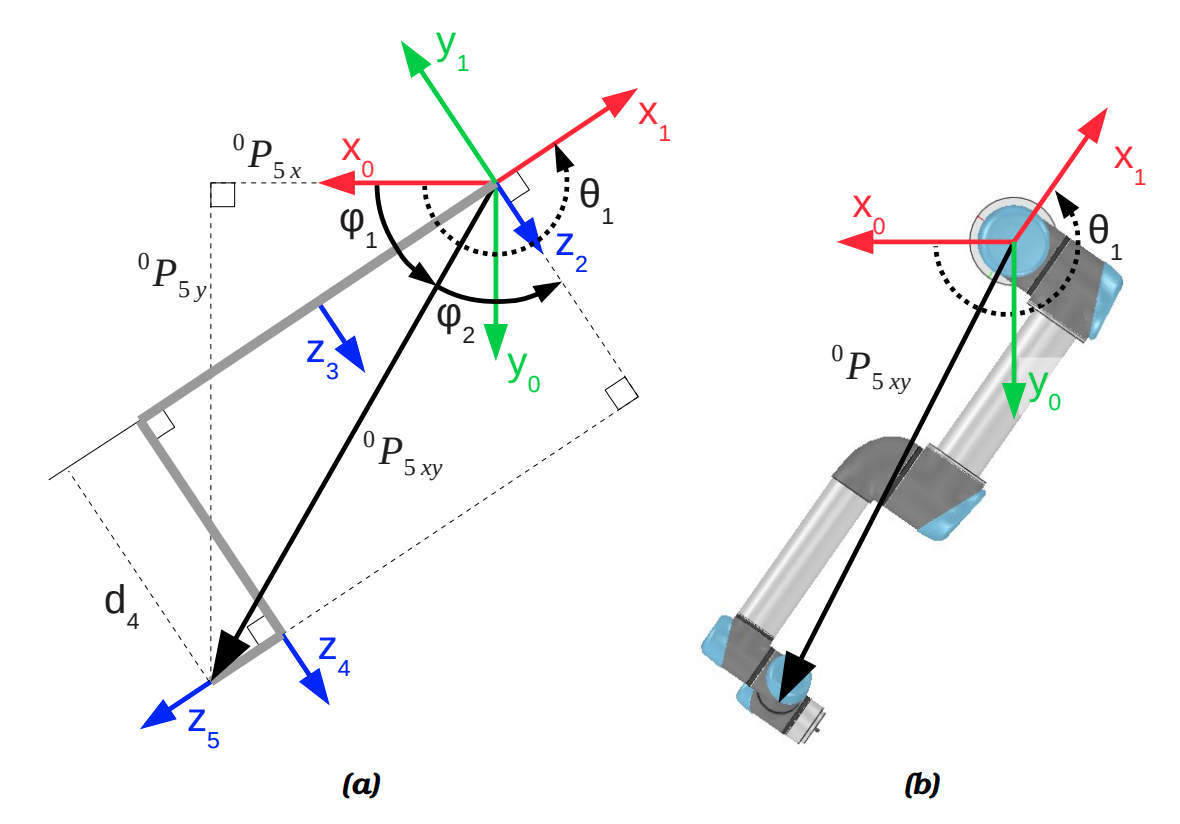
\includegraphics[width = .5\textwidth]{Bilder/inv1}
    \caption{Berechnung von $\theta_1$, Betrachtung von Gelenk eins bis fünf~\cite{rasmusandersenKinematicsUR52018}}\label{fig:inv1-1}
\end{figure}

\subsubsection{2. Gelenk fünf (oberes Handgelenk)}

Im Anschluss kann $\theta_5$ bestimmt werden, da der y-Teil der Position von Gelenk 6 relativ zu Gelenk 1 ($P_{1,6y}$) nur mithilfe von $\theta_5$ und bereits bekannter Parameter $P_{0,6}$, $\theta_1$ und der DH-Parameter berechnet werden kann (siehe Abbildung~\ref{fig:inv1-2}).
Aus dieser Erkenntnis ergibt sich Gleichung~\ref{eq:inv2-1}
$P_{1,6y}$ erhält man durch die Rotation des Ursprungssystems $T_{0,6}$ um die $z_1$-Achse (Gleichung~\ref{eq:inv2-2}).
In Kombination erhält man die Gleichung für $\theta_5$ (Gleichung~\ref{eq:inv2-3}).
Dabei entstehen wiederum zwei Lösungen, die jeweils das Handgelenk ober- oder unterhalb des Arms platzieren.
\begin{equation}
    - P_{1,6y} = d_4 + d_6 \cdot \cos(\theta_5)
    \label{eq:inv2-1}
\end{equation}
\begin{equation}
    P_{1,6y} = - P_{0,6x} \cdot \sin(\theta_1) + P_{0,6y} \cdot cos(\theta_1)
    \label{eq:inv2-2}
\end{equation}
\begin{equation}
    \theta_5 = \pm \arccos \left( \frac{ P_{0,6x} \cdot \sin\theta_1 - P_{0,6y} \cdot \cos\theta_1 - d_4 }{ d_6 } \right)
    \label{eq:inv2-3}
\end{equation}
\begin{figure}[h]
    \centering
    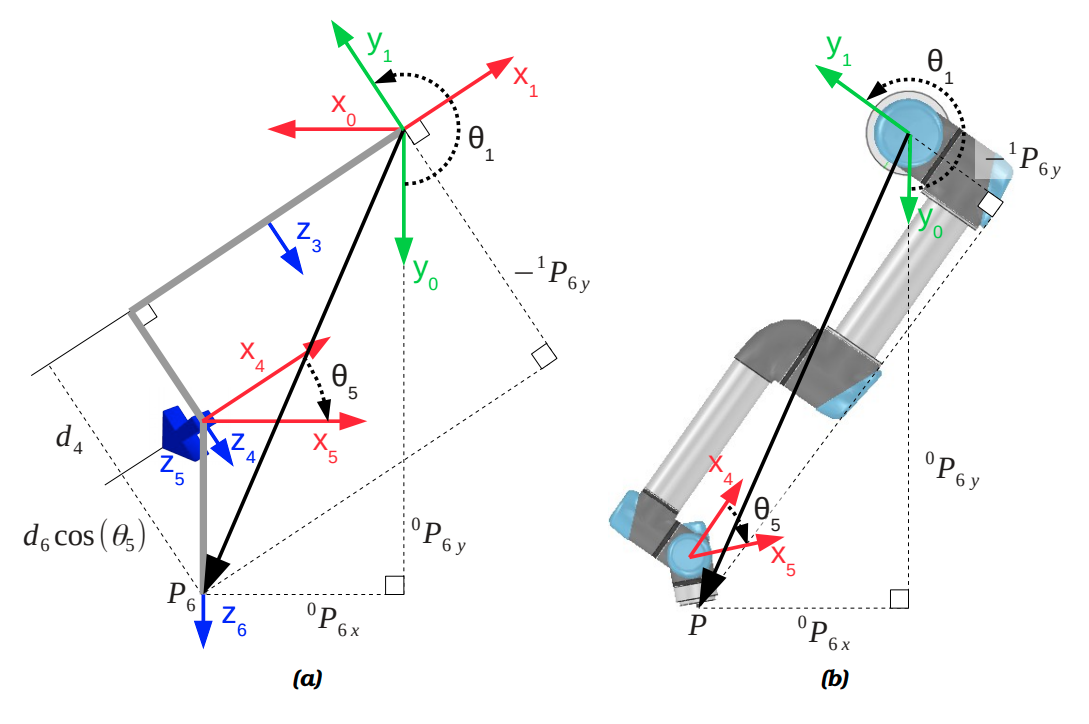
\includegraphics[width = .5\textwidth]{Bilder/inv2}
    \caption{Berechnung von $\theta_5$, Betrachtung von allen Gelenken~\cite{rasmusandersenKinematicsUR52018}}\label{fig:inv1-2}
\end{figure}

\subsubsection{3. Gelenk sechs (Endeffektor)}

Nach $\theta_1$ und $\theta_5$ wird $\theta_6$ bestimmt.
Dazu wird die Eigenschaft des UR5 herangezogen, die Z-Achsen von Gelenken zwei, drei und vier liegt stets parallel zur Y-Achse von Gelenk 1 stehen (siehe Abbildung~\ref{fig:ur5-axis}).
Deshalb kann die Y-Achse $y_1$ beschrieben von Gelenk sechs ($Y_{6,1}$) unabhängig von $\theta_{1,2,3,4}$ und kann mithilfe von sphärischen Koordinaten als $-Y_{6,1}(-\theta_6,\theta_5)$ ($-\theta_5$ als Azimuth sowie $\theta_6$ als polaren Winkel) aufgefasst werden (Abbildung~\ref{fig:inv1-3}).
Eine Umrechnung in kartesische Koordinaten ergibt deshalb Gleichung~\ref{eq:inv3-1}, wobei $Y_{6,1}$ mithilfe einer Drehung um $\theta_1$ um $z_1$ beschrieben werden kann (Gleichung~\ref{eq:inv3-2}).
$Z$ und $X$ sind hierbei jeweils Einheitsvektoren der Z- und X-Achse des jeweiligen Koordinatensystems.
Nach Gleichsetzen der x- und y-Einträge der beiden Gleichungen und anschließendem Umformen erhält man $\theta_6$ (Gleichung~\ref{eq:inv3-3}).
Dabei kann es genau eine Lösung geben.
Falls $\sin\theta_5=0$, liegt eine Singularität vor und eine Lösung kann nicht bestimmt werden.
Dies tritt auf, wenn neben den Achsen $z_2$, $z_3$ und $z_4$ auch Achse $z_6$ parallel steht.
In diesem Fall kann eine beliebige Lösung gewählt werden, im Regelfall wird $\theta_6=0$ gesetzt.

\begin{figure}[h]
    \centering
    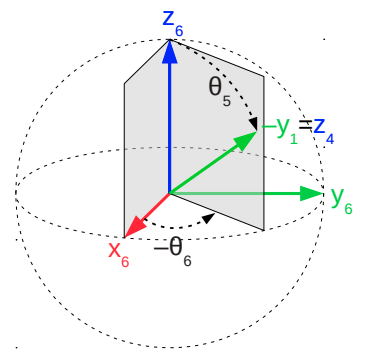
\includegraphics[width = .4\textwidth]{Bilder/inv3}
    \caption{Berechnung von $\theta_6$ mit Sphärischen Koordinaten, für Koordinatensystembeschreibung siehe Abbildung~\ref{fig:ur5-axis}~\cite{rasmusandersenKinematicsUR52018}}\label{fig:inv1-3}
\end{figure}
\begin{equation}
    Y_{6,1}=
    \begin{bmatrix}
        -\sin\theta_5 \cdot \cos\theta_6 \\ \sin\theta_5 \cdot\sin\theta_6 \\ -\cos\theta_5
    \end{bmatrix}
    \label{eq:inv3-1}
\end{equation}
\begin{equation}
    Y_{6,1}=
    -\sin\theta_1\cdot X_{6,0} + \cos\theta_1\cdot Y_{6,0}
    \label{eq:inv3-2}
\end{equation}
\begin{equation}
    \theta_6=
    \arctantwo\left(
    \frac{
        -X_{6,0y} \cdot \sin\theta_1 + Y_{6,0y} \cdot \cos\theta_1
    }{
        \sin\theta_5
    },
    \frac{
        X_{6,0x} \cdot \sin\theta_1 - Y_{6,0x} \cdot \cos\theta_1
    }{
        \sin\theta_5
    }\right)
    \label{eq:inv3-3}
\end{equation}

\subsubsection{4. Gelenk drei (Ellenbogen)}

Die verbleibenden drei Gelenke haben alle parallele Achsen und lassen sich dadurch zu einem zweidimensionalen System vereinfachen (siehe Abbildung~\ref{fig:inv1-4}, rechts).
Um $\theta_3$ zu berechnen kann der Winkel $\phi_3$ zu Hilfe genommen werden (siehe Gleichung~\ref{eq:inv4-1}).
Die Werte $a_2$, $a_3$ sind dabei die DH-Parameter der jeweiligen Gelenke und $\lvert P_{1,4xz} \rvert$ ist der Abstand zwischen Gelenk 1 und Gelenk 4, dessen relative Position bereits bekannt ist.
Aufgrund der Geometrie gilt: $\lvert P_{1,4xz} \rvert \in \lvert a_2 \pm a_3 \rvert$
Nach der Anwendung des $\arccos$ erhält man in der Regel zwei Lösungen, die der Position \enquote{Elbow Up} und \enquote{Elbow Down} entsprechen (Gleichung~\ref{eq:inv4-2}).
\begin{equation}
    \cos(\theta_3) = -cos(\phi_3) = \frac{a_2^2 + a_3^2 - \lvert P_{1,4xz}^2 \rvert}{2 a_2 a_3}   \label{eq:inv4-1}
\end{equation}
\begin{equation}
    \theta_3 = \pm \arccos \left(  \frac{a_2^2 + a_3^2 - \lvert P_{1,4xz}^2 \rvert}{2 a_2 a_3} \right)  \label{eq:inv4-2}
\end{equation}
\begin{figure}[h]
    \centering
    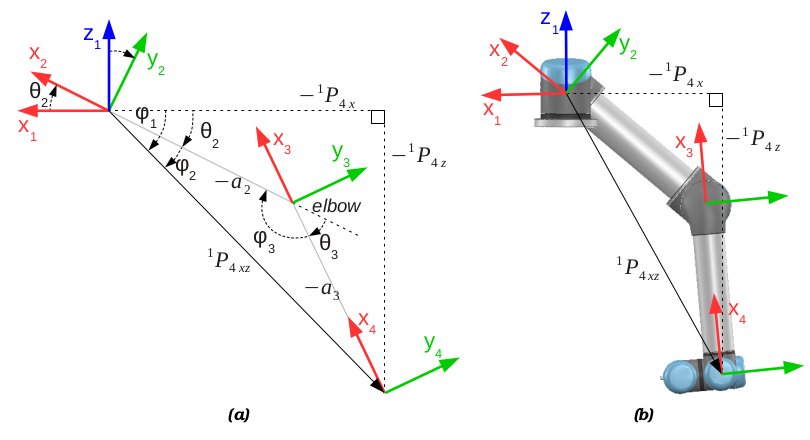
\includegraphics[width = .8\textwidth]{Bilder/inv4}
    \caption{Berechnung von $\theta_4$ durch Vereinfachung als zweidimensionales System und Bestimmung der Transformation zwischen Gelenk 1 und Gelenk 4~\cite{rasmusandersenKinematicsUR52018}}\label{fig:inv1-4}
\end{figure}

\subsubsection{5. Gelenk zwei (Schulter)}

$\theta_2$ kann mithilfe von Abbildung~\ref{fig:inv1-4} ($\theta_2 = \phi_1 - \phi_2$), sowie Gleichung~\ref{eq:inv5-2} und ~\ref{eq:inv5-3} bestimmt werden.
Nach der Substitution von $\phi_3 = \sin(\pi-\theta_3) = \sin(\theta_3)$ erhält man eine Lösung für $\theta_2$ (Gleichung~\ref{eq:inv5-4}).
%\begin{equation}
%    \label{eq:inv5-1}
%\end{equation}
\begin{equation}
    \phi_1 = \arctantwo(-P_{1,4_z}, -P_{1,4x}) \label{eq:inv5-2}
\end{equation}
\begin{equation}
    \phi_2 = \arcsin\left( \frac{-a_3\cdot \sin \phi_3}{\lvert P_{1,4xz}\rvert} \right) \label{eq:inv5-3}
\end{equation}
\begin{equation}
    \theta_2 = \phi_1 - \phi_2 =
    \arctantwo(-P_{1,4_z}, -P_{1,4x}) -
    \arcsin\left( \frac{-a_3\cdot \sin \theta_3}{\lvert P_{1,4xz}\rvert} \right)
    \label{eq:inv5-4}
\end{equation}

\subsubsection{6. Gelenk vier (unteres Handgelenk)}

Der Winkel des letzten Gelenks ist definiert als der Winkel zwischen den Achsen $x_3$ und $x_4$ um Rotationsachse $z_4$ (siehe Definition DH-Parameter, Abschnitt~\ref{sec:dh-konvention}).
Da alle anderen Winkel bereits bekannt sind, kann der letzte Winkel der ersten Spalte $X_{3,4}$ der Transformationsmatrix $T_{3,4}$ entnommen werden.
Mit den ersten beiden Werten dieser Spalte, $X_{3,4x}$ und $X_{3,4y}$, erhält man den Wert von $\theta_4$ (Gleichung~\ref{eq:inv6-1})

\begin{equation}
    \theta_4 = \arctantwo\left( X_{3,4y}, X_{3,4x} \right)    \label{eq:inv6-1}
\end{equation}

\subsubsection{Zusammenfassung}

Mithilfe der Gleichungen~\ref{eq:inv7-1} bis~\ref{eq:inv7-6} kann die Inverse Kinematik eines UR5-Roboters direkt bestimmt werden.
Dabei existieren in der Regel acht mögliche Lösungen, jeweils eine für die Gelenke sechs (Endeffektor), zwei (Schulter) und vier (unteres Handgelenk) und jeweils zwei für die Gelenke eins (Basis), drei (Ellenbogen) und fünf (oberes Handgelenk).
Falls die Achsen $z_2$, $z_3$, $z_4$ und $z_6$ parallel stehen, kann $\theta_6$ beliebig gewählt werden, sodass eine Singularität mit beliebig vielen Lösungen vorliegt.
Neben den DH-Parametern und der gewünschten Transformation des Endeffektors muss für Gleichung~\ref{eq:inv7-1} $P_{0,5}$ (Gleichung~\ref{fig:inv1-1}), für Gleichung~\ref{eq:inv7-3} die Transformation $T_{60}$, für Gleichung~\ref{eq:inv7-4} und~\ref{eq:inv7-4} die Transformation $T_{14}$ und für Gleichung~\ref{eq:inv7-6} die Transformation $T_{3,4}$ mit der Regeln aus Gleichungen~\ref{eq:inv-rule0},~\ref{eq:inv-rule1} und~\ref{eq:inv-rule2} bestimmt werden.

\begin{equation}
    \theta_1 = \arctantwo(P_{0,5y}, P_{0,5x}) \pm \arccos \left( \frac{d_4}{ \sqrt{ P_{0,5x}^2 + P_{0,5y}^2 }  } \right) + \frac{\pi}{2}
    \label{eq:inv7-1}
\end{equation}
\begin{equation}
    \theta_5 = \pm \arccos \left( \frac{ P_{0,6x} \cdot \sin\theta_1 - P_{0,6y} \cdot \cos\theta_1 - d_4 }{ d_6 } \right)
    \label{eq:inv7-2}
\end{equation}
\begin{equation}
    \theta_6 =
    \arctantwo\left(
    \frac{
        -X_{6,0y} \cdot \sin\theta_1 + Y_{6,0y} \cdot \cos\theta_1
    }{
        \sin\theta_5
    },
    \frac{
        X_{6,0x} \cdot \sin\theta_1 - Y_{6,0x} \cdot \cos\theta_1
    }{
        \sin\theta_5
    }\right)
    \label{eq:inv7-3}
\end{equation}
\begin{equation}
    \theta_3 = \pm \arccos \left(  \frac{a_2^2 + a_3^2 - \lvert P_{1,4xz}^2 \rvert}{2 a_2 a_3} \right)
    \label{eq:inv7-4}
\end{equation}
\begin{equation}
    \theta_2 = \phi_1 - \phi_2 =
    \arctantwo(-P_{1,4_z}, -P_{1,4x}) -
    \arcsin\left( \frac{-a_3\cdot \sin \theta_3}{\lvert P_{1,4xz}\rvert} \right)
    \label{eq:inv7-5}
\end{equation}
\begin{equation}
    \theta_4 = \arctantwo\left( X_{3,4y}, X_{3,4x} \right)
    \label{eq:inv7-6}
\end{equation}

Die Schritte zur Berechnung der inversen Kinematik können für das bessere Verständnis im Code ?? (Anhang referenz) direkt nachvollzogen und visualisiert werden.


\section{Singularitäten}\label{sec:singularitaten}

Wie in Abschnitt~\ref{sec:geometrische-losung} ermittelt, existiert beim UR5 genau eine Position, bei der eine Singularität vorliegt.
Singularitäten zeichnen sich dadurch aus, dass es unendlich viele Lösungen für eine bestimmte Zieltransformation gibt.
In der Regel tritt dies genau dann auf, wenn zwei Rotationsachsen parallel zueinander stehen und ihre Bewegung durch das Drehen in gegensätzliche Richtungen beliebig ausgleichen können.

In der Praxis tritt dieser Fall allerdings kaum auf, da durch kleine Rundungsfehler bei der Rechnung nur im Extremfall eine exakte Parallelität hergestellt wird.
Trotzdem sind Singularitäten problematisch, da beim Durchfahren einer solchen Position extreme Positionsänderungen der verschiedenen Gelenke erforderlich sind.
Aus diesem Grund ist es ratsam, diese Positionen möglichst zu vermeiden.
Für weitere Informationen zur Pfadplanung, siehe Abschnitt~\ref{ch:pfadplanung}.

    \cleardoublepage


\chapter{Pfadplanung}\label{ch:pfadplanung}

Bei der Pfadplanung geht es darum, eine Reihe an Konfigurationen zu berechnen, die den Weg von einer bestimmten Transformation in eine andere beschreiben.
Eine einzelne Konfiguration ist im Falle des UR5 ein Tupel mit sechs Winkeln, die die Ausrichtung der sechs Gelenke des Roboters beschreiben.

Die einfachste Form der Pfadplanung ist der kürzeste Weg zwischen zwei Punkten (Abschnitt~\ref{subsec:kurzester-weg}), die schnellste Verbindung ist immer der Weg der direkten Kinematik mit maximaler Winkelgeschwindigkeit bei der Bewegung (Abschnitt~\ref{ch:direkte-kinematik}).
Komplizierter wird es, wenn Beschränkungen im Arbeitsraum des Roboters, wie Kollisionen mit der Umgebung oder mit sich selbst, vorliegen.
In diesem Fall muss ein komplizierteres Berechnungsverfahren herangezogen werden.

In diesem Kapitel sollen die Grundlagen der Pfadplanung, sowie einige Algorithmen näher vorgestellt werden.


\section{Konfigurationsraum}\label{sec:konfigurationsraum}


Der Konfigurationsraum $\mathit{C}$ stellt die Grundlage für die Algorithmen in der Pfadplanung dar und beschreibt alle möglichen Konfigurationen, die der Roboter einnehmen kann.
Eine Konfiguration des UR5 ist dabei wie in Gleichung~\ref{eq:config-1} definiert, wobei die Winkelwerte $\theta_i$ durch ihre Maximal- und Minimalwerte des Datenblatts~\cite{universalrobotsUR5TechnicalSpecifications} von $\pm 360^{\circ}$ beschränkt sind.
Gleichsam existieren Konfigurationen innerhalb dieser Menge $\mathit{O}\in\mathit{C}$, die Kollisionen beschreiben.
Darunter zählen Konfigurationen, bei denen sich der Roboter selbst im Weg steht, sowie welche, bei denen der Untergrund oder statische Hindernisse eine erfolgreiche Ausführung der Bewegung verhindern.
Der für die Pfadplanung relevante Bereich ist demzufolge der in Gleichung~\ref{eq:config-2} beschriebene Menge $\mathit{C}_{free}$, der freie Konfigurationsraum, dessen Konfigurationen den Bereich beschreiben, durch den Roboter sich bewegen kann.

\begin{equation}
    \mathit{C} = \left\{ \left( \theta_1,\dots,\theta_6 \right) \in \theta_1\times\dots\times\theta_6 \mid \theta_i \in \left[ -2\pi, 2\pi \right]\right\}
    \label{eq:config-1}
\end{equation}
\begin{equation}
    \mathit{C}_{free} = \mathit{C}\backslash\mathit{O}
    \label{eq:config-2}
\end{equation}

Je nach Algorithmus muss der Konfigurationsraum allerdings nicht im vorhinein berechnet werden.
Um den Kollisionsraum abzubilden wurde der Roboter in dieser Arbeit mit Kugeln und Zylindern in den Dimensionen des UR5 approximiert und in fünf-Grad Schritten jede Position auf Eigenkollision getestet, damit Pfadplanungsalgorithmen schneller auf ihre Funktionsweise hin untersucht werden können.

?? Code

??Quelle

% todo berechnung/beschreibung von collision detection mit bb / trees
https://www.geometrictools.com/Documentation/DynamicCollisionDetection.pdf


\section{Berechnungsmethoden}
%
%\subsection{Kürzester Weg}\label{subsec:kurzester-weg}
Im einfachsten Fall soll der Roboter auf kürzestem Weg in eine Zielposition fahren.
Dabei wird die Wegstrecke meist linear in mehrere Zwischentransformationen zwischen zwei oder mehr Transformationen $T_1$ und $T_2$ aufgeteilt.
Für die Translation von Punkt $P_1$ und Punkt $P_2$ kann für jeden Schritt ein Faktor $t \in \left[0,1\right]$ multipliziert werden (Gleichung~\ref{eq:shortest-path-1}).
Zwischen zwei Rotationen $R_1$ und $R_2$ wird in der Regel der sog.\ Slerp verwendet (Gleichung~\ref{eq:shortest-path-2}).
Dabei müssen die Rotationen der allerdings erst in Quaternionen $Q_1$ und $Q_2$ umgerechnet werden.
Zu beachten sind zudem die Rechenregeln der Quaternionen, die hier nicht näher erklärt werden.

\begin{equation}
    P_{t} = P_0 + \left( P_1 - P_0 \right) \cdot t
    \label{eq:shortest-path-1}
\end{equation}
\begin{equation}
    Q_{t} = Q_1 \cdot \left( Q_1^{-1} \cdot Q_2 \right)^t
    \label{eq:shortest-path-2}
\end{equation}

Die resultierende Liste an Endeffektor-Transformationen muss dann in den Konfigurationsraum des Roboters übersetzt werden.
Beim UR5 gibt es, wie in Abschnitt~\ref{sec:geometrische-losung} berechnet, für jede Zwischentransformation oftmals bis zu acht, oder in einer Singularität sogar unendlich viele Stellungen für die Gelenke.
Um einen geeigneten Pfad durch den Konfigurationsraum zu nehmen und die Selbstkollision sowie das Erreichen von Winkelbegrenzungen zu vermeiden, sollte deshalb ein Pfadplanungsalgorithmus zu Hilfe genommen werden.

?? Quelle

\subsection{Zellendekomposition}\label{subsec:zellendekomposition}
?? Quelle

In der Zellendekomposition wird der freie Konfigurationsraum $C_{free}$ in kleinere Felder, sog.\ Zellen unterteilt.
Zwei Konfigurationen liegen genau dann in der gleichen Zelle, falls ein Übergang zwischen den beiden Zuständen kollisionsfrei möglich ist und zwei benachbarte Zellen müssen über einen einfachen Pfad miteinander kollisionsfrei verbunden sein.
Dies setzt konvexe Zellen voraus, bei denen jeder Punkt innerhalb der Zelle jeden anderen erreichen kann.
Auf Basis dieser Gruppierungen kann dann ein Konnektivitätsgraph oder eine Roadmap erstellt werden.
Als Datenstruktur kann ein KD-Tree verwendet werden, der ein Konfigurationsraum als Baum so abbildet, dass Abstände und benachbarte Zellen zügig berechnet werden können.
Im zweidimensionalen Raum werden hierfür die Positionen und Dimensionen von Quadraten sowie dessen Nachbarn gespeichert.

Diese direkte Berechnung der Zellenstruktur ist im sechsdimensionalen Fall des UR5 allerdings nichttrival und aufwändig.
Aus diesem Grund und für die schnellere Berechnung wird deshalb oftmals eine approximierte Lösung aus einem Sampling-Verfahren bevorzugt.

\subsection{Sampling-Verfahren}
?? Quelle

In Sampling-basierten Verfahren wird das Gruppieren aller Konfigurationen in konkave Zellen übersprungen und stattdessen nur einzelne, benötigte Konfigurationen auf Kollision geprüft.
Das bedeutet, dass nicht, wie in Abschnitt~\ref{subsec:zellendekomposition} alle Lösungen für alle Probleme generalisiert werden sollen, sondern eine einzelne Lösung für ein einzelnes Problem gesucht ist.
Bedingung dafür ist allerdings eine Möglichkeit, eine Konfiguration schnell auf Kollisionsfreiheit zu überprüfen.
Insofern der Konfigurationsraum wie in Abschnitt~\ref{sec:konfigurationsraum} schon zuvor berechnet wurde, kann alternativ ein Lookup-Table verwendet werden.
Dabei kann zwischen Single- und Multi-Query-Verfahren unterschieden werden.

\subsubsection{Single-Query}

Bei Single-Query-Verfahren wird für jede Abfrage ein neuer Weg gesucht, bei Multi-Query-Verfahren werden vergangene Anfragen als Hilfestellung für neue Anfragen genutzt und so eine Roadmap erzeugt.
Üblicherweise wird beim Single-Query-Verfahren mit Startkonfiguration $q_a$ und Zielkonfiguration $q_b$ wie folgt vorgegangen:
\begin{enumerate}
    \item Initalisierung eines Graphens $G(V, E)$ mit Knoten mit $V=\left\{ q_a, q_b \right\}$ und $E=\left\{  \right\}$
    \item Auswahl eines Expansionsknotens aus $V$ mit einem gewählten Algorithmus
    \item Berechnung eines neuen Knotens und einer Kante mit einem gewählten Algorithmus (inklusive Kollisionsüberprüfung)
    \item Erweiterung des Graphens mit zuvor gefundenem Knoten und neuer Kante (falls möglich).
    \item Prüfe auf Lösung in G (Verbindung von Start und Zielknoten) oder wiederhole ab 2.
\end{enumerate}

Zudem kann der Algorithmus auf zwei oder mehr Suchbäume ausgeweitet werden, die sich nach einiger Zeit in der Mitte treffen.
Dazu wird dann in den Schritten 2\-4 der verwendete Baum zufällig ausgewählt.

Der \ac{rrt} ist ein häufig verwendeter Suchbaum in diesem Kontext.
Hier wird zunächst wie in 3.\ eine neue Konfiguration zufällig gewählt und ab dem nächsten Knoten im Graphen eine Schrittweite in Richtung dieser Konfiguration gegangen.
Um einen Bias gegenüber der Zielkonfiguration zu erzeugen, kann zudem mit einer gewissen Wahrscheinlichkeit der zufällig gewählte Knoten mit dem tatsächlichen Zielknoten ersetzt werden.
Bei RRT$^*$ wird bei der Erweiterung zusätzlich auf andere Verbindungen des Graphens zum neu berechneten Knoten geprüft, was die Länge der kürzesten Verbindung zwischen Start und Ziel noch einmal minimiert.
Die kürzeste Verbindung kann beispielsweise mithilfe von A$^*$ oder Dijkstra ermittelt werden.

\subsubsection{Multi-Query}
Bei Multi-Query Verfahren können bereits berechnete Kanten des aufgebauten Graphens wiederverwendet werden.
Im Probabilistic-Roadmap-Algorithmus werden in einem ersten Schritt n zufällige Knotenpunkte erzeugt und dann mit ihren nächsten Nachbarn verbunden, insofern keine Kollision vorliegt.
Im Anschluss werden Start- und Zielknoten ergänzt und ebenfalls Nachbarn als Kanten im Graphen hinzugefügt.
Am Ende kann dann wieder mithilfe von A$^*$ oder Dijkstra ein kürzester Weg ermittelt werden.


??

%Single-Query
%Unidirektional vs.\ Bidirektional
%RRT
%biased / unbiased to exploration
%Q-space muss nicht vollständig bekannt sein
%RRT*
%Multi-Query
%Probabilistic Roadmaps
Potentialfeldmethode / Gradientenverfahren
Genetische Algorithmen


\section{Constraints und Praxisbezug}
Kinematisch (Winkelbegrenzung)
Dynamisch (Geschwindigkeit)
Einbezug der Constraints in den Algorithmen
Praxis: OMPL (MoveIt+ ROS / Copelliasim Plugin)


%    \cleardoublepage


\chapter{Trajektorienplanung}


\section{Profile}

Trapez, 7-Segment


\section{Synchronität}

Vollsynchron, Teilsynchron, Asynchron


\section{Mehrsegment-Trajektorien}

Ggf besser in Pfadplanung ??

Mehrsegment-Trajektorien (z.B. Bezier, Überschleifen)

    \cleardoublepage
\chapter{Fazit und Ausblick}

Mit den erläuterten Methoden kann ein kollisionsfreier Pfad zwischen der momentanen Position und Stellung des Roboters zu einem erreichbaren Zielpunkt auf zwei verschiedene Weisen berechnet werden.
Zum einen kann der kürzeste Weg für den Greifer zwischen den beiden Positionen gefahren werden.
Dabei werden für alle Zwischenpunkte mögliche Kollisionen und Übergänge in die nächste Konfiguration ermittelt und im Anschluss der kürzeste Weg in den übrigen Wegpunkten als Liste von Zwischenkonfigurationen ausgegeben.
Des Weiteren kann der direkte Weg gefahren werden, bei dem sich jedes Gelenk mit konstanter Winkelgeschwindigkeit vorwärts oder rückwärts zu den acht möglichen Zielstellungen bewegt.
Dabei bewegt sich der Greifer in der kürzesten der bis zu 512 Lösungen meist in einem Bogen zum Ziel.

Im nächsten Schritt kann nun ein Übergang in die Praxis erfolgen.
Hierzu muss das Programm in die Steuerung des Roboters integriert werden und in Zukunft die Pfadplanung des UR5 ersetzen.
Es sollte zudem untersucht werden, ob die implementierten Methoden bereits in OMPL (ROS mit MoveIt oder CopelliaSim Plugin) existieren und ob die hier eingesetzte Kollisionsbibliothek für den UR5 besser mit einem Kollisionstest des verwendeten Frameworks ersetzt werden sollte.
%    \input{006_Konzept}
%    \input{007_Umsetzung}
%    \input{008_Verwendung}
%    \input{009_Ausblick}
%%%%%%%%%%%%%%%%%%%%%%%%%%%%%%%%%%%%%%%%%%%%%%%%%%%%%%%%%%%%%%%%%%%%%%%%%
    \cleardoublepage
    \printbibliography    % Lit.verzeichnis
%    \input{198_Anhang}
    \chapter*{Erklärung}
Die vorliegende Arbeit habe ich selbstständig ohne Benutzung anderer als der
angegebenen Quellen angefertigt. Alle Stellen, die wörtlich oder sinngemäß
aus veröffentlichten Quellen entnommen wurden, sind als solche
kenntlich gemacht. Die Arbeit ist in gleicher oder ähnlicher Form oder
auszugsweise im Rahmen einer oder anderer Prüfungen noch nicht vorgelegt
worden.
\\[2cm]
Augsburg, den \abgabedatum\hfill \namedesautors

%%%%%%%%%%%%%%%%%%%%%%%%%%%%%%%%%%%%%%%%%%%%%%%%%%%%%%%%%%%%%%%%%%%%%%%%%
\end{document}
%%%%%%%%%%%%%%%%%%%%%%%%%%%%%%%%%%%%%%%%%%%%%%%%%%%%%%%%%%%%%%%%%%%%%%%%%
